\chapter{verwandte Arbeiten}
\label{relatedWork}

Da GraphQL eine stetig wachsende Beliebtheit verzeichnet \cite{graphql-growing-report}[vgl. Language Features] steigt auch der Bedarf und das Interesse an Testmethoden.
Aktuell gibt es für GraphQL noch eine Lücke an produktionsreifen Testtools, insbesondere automatischen Testtools.
Eine wachsende Anzahl an research-tools beziehungsweise untersuchten Methoden ist allerdings zu verzeichnen.
In diesem Kapitel sollen diese Methoden benannt werden und Verwandheiten, Unterschiede oder thematische Überschnitte von dieser und anderen Arbeiten benannt werden.

\section{Property Based Testing}

In ''Automatic Property-based Testing of GraphQL APIs''\cite{property-based-testing} wird der Ansatz des Property-based Testing verfolgt, um Integrationstests zu erstellen.
Property-based Testing ist laut dem Paper heute Synonym mit "Random Testing"\cite{property-based-testing}[vgl. 2B] wobei zufällig hierbei meint,dass die Eingabedaten und Routen zufällig generiert werden.
Wie Eingangs schon erwähnt, hat die Methode einige Limitierungen.
Wir wollen diese hier noch einmal aufgreifen und vertiefen.
Der allgemeine Funktionsablauf der Testgenerierung laut Paper ist wie folgt:

\begin{center}
    \begin{itemize}
        \item[1.] Vom Schema, generiere Typ-Spezifikationen
        \item[2.] Generiere einen Generator der zufällig eine Liste an Query-Objekten erstellen kann
        \item[3.] Generiere n Querys
        \item[4.] Transformiere die Queries in GraphQL-Format
        \item[5.] Führe die Queries auf dem SUT (system under test) aus
        \item[6.] Evaluiere die Ergebnisse auf ihre Properties
    \end{itemize}[\cite{property-based-testing}[vgl. 3. Proposed Method]]
\end{center}

Insbesondere Punkt 2. und Punkt 6. weisen Verbesserungsbedarf auf.
Punkt 2 wird auch der Hauptunterscheidungspunkt beider Arbeiten sein, denn hier sind dann zwei gänzlich unterschiedliche Konzepte am Werk.
Dieser ist beim Property-Based Testing nämlich ein Query-Generator der mithilfe der Clojure-Bilbiothek Serene\cite{clojureserene}
Clojure.Specs\cite{clojurespec} generiert und diese Clojure.Specs\cite{clojurespec} dann nutzt um mit der Clojure-Bilbiothek Malli\cite{clojuremalli} dann Daten für die Testqueries zu generieren.
Unsere herangehensweise wird sich hiervon gänzlich unterscheiden.
Im Sinne von Property-based Testing ist diese Herangehensweise allerdings eine sehr sinnvolle gewesen da Malli\cite{clojuremalli} de-facto Standard
für Property-based Testing in der Clojure-Welt ist.
Geht man jedoch davon aus, dass das Ziel eine ideale Überdeckung des Graphens jeder größe und jeder Struktur ist, so
ist diese herangehensweise nicht die beste.\cite{property-based-testing}[vgl. 3C]
Laut dem Paper gilt ''ein größeres und mehr rekursives (GraphQL)-Schema würde nicht skalieren und der (zufällig) iterative Ansatz ist besser als eine Breitensuche''\cite{property-based-testing}[vgl. 3C].
Diese Behauptung betrachten wir als falsch und behaupten, dass es besser möglich ist.
Dies zu zeigen bleibt Gegenstand der folgenden Arbeit.


\section{heuristisch suchenbasiertes Testen}

EvoMaster\cite{evo-master} ist ein Open-Source Tool welches sich automatisiertes Testen von Rest-APIs und GraphQL APIs zur Aufgabe gemacht hat.
Aktuell kann durch EvoMaster sowohl WhiteBox Testing als auch BlackBox Testing durchgeführt werden jedoch ist ein
Whitebox Test mittels Vanilla-EvoMaster nur für Rest-APIs möglich die mit der JVM lauffähig sind.
Im Paper ''White-Box and Black-Box Fuzzing for GraphQL APIs''\cite{belhadi2022whitebox} wurde ein System on-Top für EvoMaster
erstellt welches GraphQL Tests generieren kann.
Hierbei soll sowohl WhiteBox als auch BlackBox Testing möglich sein.
Das erstellte Framework in diesem Paper arbeitet nach folgendem Prinzip:

\begin{center}
    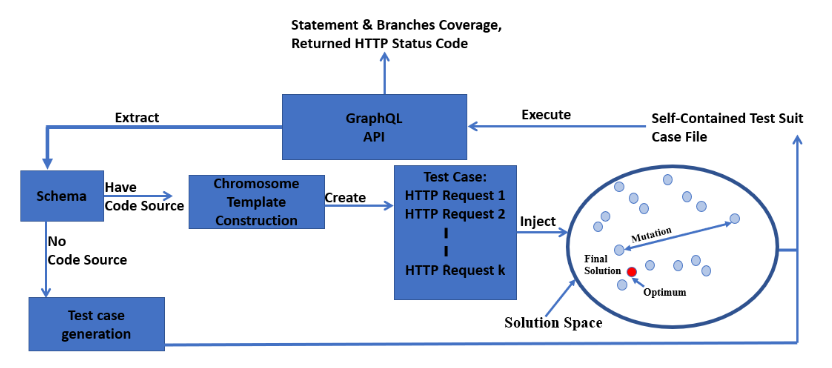
\includegraphics[width=\textwidth,height=\textheight,keepaspectratio]{content/hauptteil/relatedWork/evomaster_framework}
\end{center}

WhiteBox Testing ist möglich insofern Zugang zum GraphQL-Schema und zum Source Code der API gegeben ist.
Andernfalls ist nur BlackBox Testing möglich.
Zur Testgenerierung wird ein genetischer Algorithmus genutzt welcher die Tests generiert.
Wie dieser genetische Algorithmus genau funktioniert kann im Paper selbst nachgelesen werden\cite{belhadi2022whitebox}.
Im Vergleich mit unserer geplanten Arbeit mittels des Prime-Path-Algorithmus ergeben sich einige Unterschiede, diese sind
unter anderem: Nutzung eines evolutionären Algorithmus Many-Independent-Objective (MIO).
Im Paper selbst wird davon ausgegangen, dass andere evolutionäre Algorithmen unter Umständen passender wären als der MIO Algorithmus
für die Testgenerierung.
Jedoch ist ein evolutionärer Algorithmus auch immer ein stochastisch, heuristisch sich dem Optimum annähernder Algorithmus. (Beleg hierfür)
Im Gegensatz dazu ist der Ansatz dieser Arbeit ein iterativer Algorithmus der ideale Überdeckungen auf direkte Art bietet
und im ersten Durchlauf direkt sein ideales Ergebnis ermittelt.
Die ideale Lösung bezieht sich hierbei auf bestimmte Code-Coverage Kriterien die durch unseren Algorithmus erfüllt werden.
Inwiefern der evolutionäre Algorithmus diese Kriterien erfüllt bleibt offen, es ist jedoch davon auszugehen, dass er sich einer idealen Lösung dieser Kriterien nur
annähert da er eben ein stochastischer Algorithmus ist. (beleg oder Quelle)

\section{Deviation Testing}

Da GraphQL dynamisch auf Anfragen reagiert und es somit möglich ist, in seiner Anfrage einzelne Felder mit einzubeziehen
oder auch auszuschließen ist dies im Grunde genommen ein einzelner Test-Case.
Im Paper \" Deviation Testing: A Test Case Generation Technique for GraphQL APIs" wird diese Gegebenheit benutzt und
aus einer selbstdefinierten Query werden hier einzelne Test-Cases gebildet. Ein solcher Test macht je nach Implementierung
der GraphQL-Resolver druchaus Sinn, da im Backend Felder durchaus zusammenhängen können und es Bugs geben kann wenn
Resolver fehlerhaft definiert sind. z.B. könnte folgende Definition zu solchen Fehlern führen:

(hier BSP mit Code einfügen)

Da Deviation Testing jedoch nur bestehende Tests erweitert um mögliche Felder mitzutesten werden hier keine neuen Tests generiert.
Durch Deviation Testing werden bestehende Tests nur erweitert allerdings muss eine Edge-Coverage gegeben sein damit diese Arbeit
ein zufriedenstellendes Ergebnis erzeugt. Eine Edge-Coverage in einem komplexen Graphen ist allerdings sehr wahrscheinlich
schwer umsetzbar mit manuellem Test schreiben. Eine Paarung von Edge-Coverage mit Deviation-Testing wäre sicherlich Interessant.
Genau so wäre es interessant Deviation Testing als Teil unserer Arbeit zu nutzen indem mit diesem Tool die Tests erweitert werden.
(initialer Plan war es, einfach immer alle Felder eines Nodes zu testen, hierdurch wäre es möglich auch alle Varianten noch zu testen)

\section{Query Harvesting}

Klassisches Testen von Anwendungen beeinhaltet, dass möglichst das komplette System getestet wird bevor es verwendet wird.
Im Paper "Harvesting Production GraphQL Queries to Detect Schema Faults" wird ein gänzlich anderer Ansatz verfolgt.
Hierbei ist es nicht wichtig die gesamte GraphQL-API vor der Veröffentlichung zu testen sondern
echte Queries die in Production ausgeführt werden zu sammeln.
Der Ansatz der hierbei verfolgt wird begründet sich daraus,
dass ein Testraum für GraphQL potentiell unendlich sein kann und es sehr wahrscheinlich ist, dass nur ein kleiner
Teil der API wirklich intensiv genutzt wird, sodass auch nur dieser Teil wirklich stark durch Tests abgedeckt werden muss.
AutoGraphQL läuft hierbei in zwei Phasen wobei in der ersten Phase alle einzigartigen Anfragen geloggt werden.
In der zweiten Phase werden dann aus den geloggten Anfragen Tests generiert.
Hierbei wird für jede geloggte Query genau ein Test-Case erstellt.
Bei dieser Art des Testens wird insbesondere darauf Wert gelegt, dass es keine Fehler im GraphQL Schema gibt.
Dies ist ein wichtiger Teil um GraphQL-API's zu testen allerdings noch kein vollständiger Test denn hier wird außer Acht gelassen,
dass eine Query konform zum GraphQL-Schema sein kann aber trotzdem falsch indem zum Beispiel falsche Daten zurückgegeben werden
durch falsche Referenzierung oder ähnlichem.
In dem zu entwickelndem Tool sollten alle Querys die von AutoGraphQL geloggt werden auch berücksichtig werden da sie durch
den Prime-Path Algorithmus auch ermittelt werden.
Es kann allerdings sinnvoll sein AutoGraphQL als Monitoring-Software mitlaufen zu lassen und weitere etwaige Fehler hiermit zu loggen
und automatisch daraus Test-Cases erstellen zu können damit zukünftig keine Fehler dieser Art mehr passieren.

\section{Vergleich der Arbeiten}
Folgender Vergleich soll die verwandten Arbeiten noch einmal kurz einordnen.

\newcolumntype{C}{>{\Centering\arraybackslash}X}
\begin{center}
    \begin{table}[!hbt]
        \begin{tabularx}{\textwidth}{|C|C|C|C|C|C|}
            \hline
            \textbf{ Arbeit / Kriterium} & \textbf{Property Based Testing} & \textbf{heuristisch suchenbasiertes Testen} & \textbf{Deviation-Testing} & \textbf{Query Harvesting} \\
            \hline
            Generierungsart & Zufallsbasierte Routengenerierung & Heuristische Suche & Erweiterung von bestehenden Tests & Tracken von Querys und daraus Tests generieren \\
            \hline
            Überdeckung & Zufällig, stark abhängig von Schema  & abhängig ob Zugang zu Source Code, Zufällig aber optimaler & stark abhängig von selbst geschriebenen Tests  & stark Abhängig von User-requests  \\
            \hline
            Orakel & simples Raten & mit Source Code: Analyse & Aus entwickelten Tests &  Aus gestellten Querys \\
            \hline
            Ausführzeit & vor Prod & vor Prod & vor Prod & Verifikation / Wartung \\
            \hline
            Use-Case & allgemeines Testen & allgemeines Testen & allgemeines Testen & Testen bei Code-Änderung \\
            \hline
        \end{tabularx}
    \end{table}
\end{center}

\section{Andere Arbeiten}
Hier ist eine kurze Übersicht über andere Arbeiten, dieses Kapitel ist sehr unwahrscheinlich in einer Abgabeversion.
Es dient eher als Notizensammlung in einer hübscheren Form.

\subsection{Empirical Study of GraphQL Schemas}
Eine umfangreiche Untersuchung von Praktiken in GraphQL. Unterteilt in verschiedene Metriken wie z.B.
Anzahl der Objekttypen, Querys etc.
Interessant ist allerdings die Untersuchung von zyklischen Schemas. Insbesondere, wie groß diese Zyklen
werden können und wie sie begrenzt werden. Dies ist interessant für spätere Auswertungen. Allerdings bringt
diese Arbeit nicht viel für das direkte Testen.

\subsection{LinGBM Performance Benchmark to Build GraphQL Servers}
Eher eine Untersuchung wie GraphQL-APIs unter Last performen bzw. wie Effizient sie sind.
Der benutzte Query-Generator kann interessant sein aber es ist schwer einschätzbar wie dieser in unserem Kontext genutzt werden
kann.

\subsection{GraphQL A Systematic Mapping Study}
Richtig gute Übersicht wie GraphQL "Unter der Haube" funktioniert


